\documentclass[class=report,crop=false]{standalone}
\usepackage{standalone}
\usepackage{import}

\subimport{../preamble/}{basic.tex}

\subimport{../preamble/}{tikz.tex}

\begin{document}

\chapter{定义对照\\Table of Definitions}

% If there is any demand for sorting those items,
% do it by an external tool.

\section{抽象代数\\Abstract Algebra}

\section{集合论\\Set Theory}

参考资料:
\begin{enumerate}
	\item \textit{Algebra Chapter 0} (2nd printing) By Paolo Aluffi.
\end{enumerate}

\begin{defbox}{set}{集合}
	Todo...
\end{defbox}

\begin{defbox}{naive set theory}{朴素集合论}
	Todo...
\end{defbox}

\begin{defbox}{subset}{子集}
	Todo...
\end{defbox}

\begin{defbox}{union ($\cup$)}{并集}
	Todo...
\end{defbox}

\begin{defbox}{intersection ($\cap$)}{交集}
	Todo...
\end{defbox}

\begin{defbox}{difference ($\setminus$ or $\diagdown $)}{差集}
	Todo...
\end{defbox}

\begin{defbox}{disjoint union}{不交并}
	Todo...
\end{defbox}

\begin{defbox}{(Cartesian) product}{笛卡尔积}
	Todo...
\end{defbox}

\section{拓扑学\\Topology}

\mydefboxillus{interior}{内部}{
	$E^\circ=\left\lbrace\boldsymbol{x}\relmiddle|\exists\delta>0,\ U(\boldsymbol{x},\,\delta)\subset E\right\rbrace$.

	$E^\circ=\left\lbrace\boldsymbol{x}\relmiddle|\exists\delta>0,\ U(\boldsymbol{x},\,\delta)\cap E^c=\varnothing\right\rbrace$.
}{
	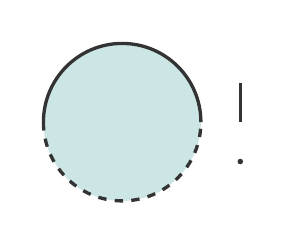
\begin{tikzpicture}[very thick]
		\fill[color=white] (-1.2,-1.2) rectangle (1.8,1.2);
		\fill[color=teal!20] (0,0) circle[radius=1];
		\draw[color=black!80] (1,0) arc[radius=1,start angle=0,end angle=180];
		\draw[color=black!80,dashed] (-1,0) arc[radius=1,start angle=180,end angle=360];
		\draw[color=black!80] (1.5,0.5) -- (1.5,0);
		\fill[color=black!80] (1.5,-0.5) circle[radius=1pt];
	\end{tikzpicture}
}

\mydefboxillus{exterior}{外部}{
	$(E^c)^\circ=\left\lbrace\boldsymbol{x}\relmiddle|\exists\delta>0,\ U(\boldsymbol{x},\,\delta)\cap E=\varnothing\right\rbrace$.

	$(E^c)^\circ=\left\lbrace\boldsymbol{x}\relmiddle|\exists\delta>0,\ U(\boldsymbol{x},\,\delta)\subset E^c\right\rbrace$.
}{
	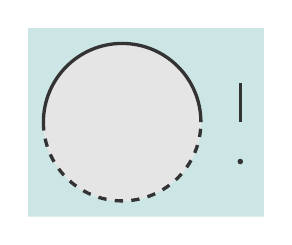
\begin{tikzpicture}[very thick]
		\fill[color=white] (-1.2,-1.2) rectangle (1.8,1.2);
		\begin{scope}
			\clip
				(-1.2,-1.2) rectangle (1.8,1.2)
				(0,0) circle[radius=1]
			;
			\fill[color=teal!20] (-1.2,-1.2) rectangle (1.8,1.2);
		\end{scope}
		\fill[color=black!10] (0,0) circle[radius=1];
		\draw[color=black!80] (1,0) arc[radius=1,start angle=0,end angle=180];
		\draw[color=black!80,dashed] (-1,0) arc[radius=1,start angle=180,end angle=360];
		\draw[color=black!80] (1.5,0.5) -- (1.5,0);
		\fill[color=black!80] (1.5,-0.5) circle[radius=1pt];
	\end{tikzpicture}
}

\mydefboxillus{boundary}{边界}{
	$\partial E=\left\lbrace\boldsymbol{x}\relmiddle|\forall\delta>0,\ (U(\boldsymbol{x},\,\delta)\cap E\neq\varnothing)\wedge(U(\boldsymbol{x},\,\delta)\cap E^c\neq\varnothing)\right\rbrace$.

	$\partial E=\mathbb{R}^n\setminus(E^\circ\cup(E^c)^\circ)$.
}{
	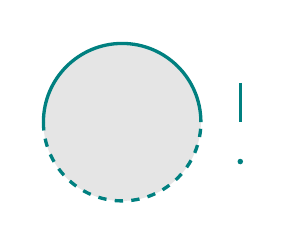
\begin{tikzpicture}[very thick]
		\fill[color=white] (-1.2,-1.2) rectangle (1.8,1.2);
		\fill[color=black!10] (0,0) circle[radius=1];
		\draw[color=teal] (1,0) arc[radius=1,start angle=0,end angle=180];
		\draw[color=teal,dashed] (-1,0) arc[radius=1,start angle=180,end angle=360];
		\draw[color=teal] (1.5,0.5) -- (1.5,0);
		\fill[color=teal] (1.5,-0.5) circle[radius=1pt];
	\end{tikzpicture}
}

\end{document}